% GNUPLOT: LaTeX picture with Postscript
\begingroup
  \makeatletter
  \providecommand\color[2][]{%
    \GenericError{(gnuplot) \space\space\space\@spaces}{%
      Package color not loaded in conjunction with
      terminal option `colourtext'%
    }{See the gnuplot documentation for explanation.%
    }{Either use 'blacktext' in gnuplot or load the package
      color.sty in LaTeX.}%
    \renewcommand\color[2][]{}%
  }%
  \providecommand\includegraphics[2][]{%
    \GenericError{(gnuplot) \space\space\space\@spaces}{%
      Package graphicx or graphics not loaded%
    }{See the gnuplot documentation for explanation.%
    }{The gnuplot epslatex terminal needs graphicx.sty or graphics.sty.}%
    \renewcommand\includegraphics[2][]{}%
  }%
  \providecommand\rotatebox[2]{#2}%
  \@ifundefined{ifGPcolor}{%
    \newif\ifGPcolor
    \GPcolortrue
  }{}%
  \@ifundefined{ifGPblacktext}{%
    \newif\ifGPblacktext
    \GPblacktextfalse
  }{}%
  % define a \g@addto@macro without @ in the name:
  \let\gplgaddtomacro\g@addto@macro
  % define empty templates for all commands taking text:
  \gdef\gplbacktext{}%
  \gdef\gplfronttext{}%
  \makeatother
  \ifGPblacktext
    % no textcolor at all
    \def\colorrgb#1{}%
    \def\colorgray#1{}%
  \else
    % gray or color?
    \ifGPcolor
      \def\colorrgb#1{\color[rgb]{#1}}%
      \def\colorgray#1{\color[gray]{#1}}%
      \expandafter\def\csname LTw\endcsname{\color{white}}%
      \expandafter\def\csname LTb\endcsname{\color{black}}%
      \expandafter\def\csname LTa\endcsname{\color{black}}%
      \expandafter\def\csname LT0\endcsname{\color[rgb]{1,0,0}}%
      \expandafter\def\csname LT1\endcsname{\color[rgb]{0,1,0}}%
      \expandafter\def\csname LT2\endcsname{\color[rgb]{0,0,1}}%
      \expandafter\def\csname LT3\endcsname{\color[rgb]{1,0,1}}%
      \expandafter\def\csname LT4\endcsname{\color[rgb]{0,1,1}}%
      \expandafter\def\csname LT5\endcsname{\color[rgb]{1,1,0}}%
      \expandafter\def\csname LT6\endcsname{\color[rgb]{0,0,0}}%
      \expandafter\def\csname LT7\endcsname{\color[rgb]{1,0.3,0}}%
      \expandafter\def\csname LT8\endcsname{\color[rgb]{0.5,0.5,0.5}}%
    \else
      % gray
      \def\colorrgb#1{\color{black}}%
      \def\colorgray#1{\color[gray]{#1}}%
      \expandafter\def\csname LTw\endcsname{\color{white}}%
      \expandafter\def\csname LTb\endcsname{\color{black}}%
      \expandafter\def\csname LTa\endcsname{\color{black}}%
      \expandafter\def\csname LT0\endcsname{\color{black}}%
      \expandafter\def\csname LT1\endcsname{\color{black}}%
      \expandafter\def\csname LT2\endcsname{\color{black}}%
      \expandafter\def\csname LT3\endcsname{\color{black}}%
      \expandafter\def\csname LT4\endcsname{\color{black}}%
      \expandafter\def\csname LT5\endcsname{\color{black}}%
      \expandafter\def\csname LT6\endcsname{\color{black}}%
      \expandafter\def\csname LT7\endcsname{\color{black}}%
      \expandafter\def\csname LT8\endcsname{\color{black}}%
    \fi
  \fi
    \setlength{\unitlength}{0.0500bp}%
    \ifx\gptboxheight\undefined%
      \newlength{\gptboxheight}%
      \newlength{\gptboxwidth}%
      \newsavebox{\gptboxtext}%
    \fi%
    \setlength{\fboxrule}{0.5pt}%
    \setlength{\fboxsep}{1pt}%
    \definecolor{tbcol}{rgb}{1,1,1}%
\begin{picture}(5760.00,4320.00)%
    \gplgaddtomacro\gplbacktext{%
      \csname LTb\endcsname%%
      \put(946,440){\makebox(0,0)[r]{\strut{}$0$}}%
      \put(946,847){\makebox(0,0)[r]{\strut{}$500$}}%
      \put(946,1253){\makebox(0,0)[r]{\strut{}$1000$}}%
      \put(946,1660){\makebox(0,0)[r]{\strut{}$1500$}}%
      \put(946,2066){\makebox(0,0)[r]{\strut{}$2000$}}%
      \put(946,2473){\makebox(0,0)[r]{\strut{}$2500$}}%
      \put(946,2879){\makebox(0,0)[r]{\strut{}$3000$}}%
      \put(946,3286){\makebox(0,0)[r]{\strut{}$3500$}}%
      \put(946,3692){\makebox(0,0)[r]{\strut{}$4000$}}%
      \put(946,4099){\makebox(0,0)[r]{\strut{}$4500$}}%
      \put(1373,308){\rotatebox{-45}{\makebox(0,0)[l]{\strut{}N: 4}}}%
      \put(1668,308){\rotatebox{-45}{\makebox(0,0)[l]{\strut{}N: 8}}}%
      \put(1962,308){\rotatebox{-45}{\makebox(0,0)[l]{\strut{}N: 16}}}%
      \put(2257,308){\rotatebox{-45}{\makebox(0,0)[l]{\strut{}N: 32}}}%
      \put(2552,308){\rotatebox{-45}{\makebox(0,0)[l]{\strut{}N: 64}}}%
      \put(2847,308){\rotatebox{-45}{\makebox(0,0)[l]{\strut{}N: 128}}}%
      \put(3141,308){\rotatebox{-45}{\makebox(0,0)[l]{\strut{}N: 256}}}%
      \put(3436,308){\rotatebox{-45}{\makebox(0,0)[l]{\strut{}N: 512}}}%
      \put(3731,308){\rotatebox{-45}{\makebox(0,0)[l]{\strut{}N: 1024}}}%
      \put(4026,308){\rotatebox{-45}{\makebox(0,0)[l]{\strut{}N: 2048}}}%
      \put(4320,308){\rotatebox{-45}{\makebox(0,0)[l]{\strut{}N: 4096}}}%
      \put(4747,440){\makebox(0,0)[l]{\strut{}$0$}}%
      \put(4747,1050){\makebox(0,0)[l]{\strut{}$2$}}%
      \put(4747,1660){\makebox(0,0)[l]{\strut{}$4$}}%
      \put(4747,2270){\makebox(0,0)[l]{\strut{}$6$}}%
      \put(4747,2879){\makebox(0,0)[l]{\strut{}$8$}}%
      \put(4747,3489){\makebox(0,0)[l]{\strut{}$10$}}%
      \put(4747,4099){\makebox(0,0)[l]{\strut{}$12$}}%
    }%
    \gplgaddtomacro\gplfronttext{%
      \csname LTb\endcsname%%
      \put(209,2269){\rotatebox{-270}{\makebox(0,0){\strut{}Communication (MiB)}}}%
      \put(5253,2269){\rotatebox{-270}{\makebox(0,0){\strut{}Improvement (number of times)}}}%
      \csname LTb\endcsname%%
      \put(3322,3926){\makebox(0,0)[r]{\strut{}GMW}}%
      \csname LTb\endcsname%%
      \put(3322,3706){\makebox(0,0)[r]{\strut{}GMW (Vectorized)}}%
      \csname LTb\endcsname%%
      \put(3322,3486){\makebox(0,0)[r]{\strut{}BMR}}%
      \csname LTb\endcsname%%
      \put(3322,3266){\makebox(0,0)[r]{\strut{}BMR (Vectorized)}}%
      \csname LTb\endcsname%%
      \put(3322,3046){\makebox(0,0)[r]{\strut{}GMW Improvement}}%
      \csname LTb\endcsname%%
      \put(3322,2826){\makebox(0,0)[r]{\strut{}BMR Improvement}}%
    }%
    \gplbacktext
    \put(0,0){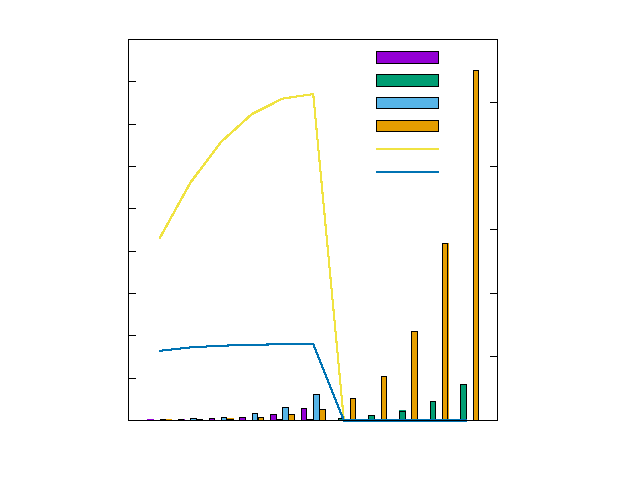
\includegraphics[width={288.00bp},height={216.00bp}]{biometric-hist-CommunicationMiB}}%
    \gplfronttext
  \end{picture}%
\endgroup
